\documentclass{beamer}
\usepackage[utf8]{inputenc}
\usepackage{listings}
\usepackage{booktabs}
\usepackage{amssymb}
\usepackage{amsmath}
\usepackage{bm}
\usepackage{enumitem}
\usepackage{hyperref}
\usepackage[export]{adjustbox}
\usepackage{svg}

\usetheme{Madrid}
\definecolor{mlpblue}{rgb}{0.1, 0.14, 0.24}

\useoutertheme{infolines} % Alternatively: miniframes, infolines, split
\useinnertheme{circles}
\usecolortheme[named=mlpblue]{structure}

\lstset{basicstyle=\footnotesize\ttfamily,breaklines=true}

%------------------------------------------------------------
%This block of code defines the information to appear in the
%Title page
\title[Contrastive Optimization]{Crossing Cross-Entropy:}

\subtitle{The Power of Provably Faithful Interpretability}

\author[Mathematical Foundations of DL] % optional
{J.~Setpal} 

\date{October 10, 2024}

\titlegraphic{
\includegraphics[width=7cm]{../shared/logo-long.pdf}}

%End of title page configuration block
%------------------------------------------------------------

%The next block of commands puts the table of contents at the 
%beginning of each section and highlights the current section:

\AtBeginSection[]
{
  \begin{frame}
    \frametitle{Outline}
    \tableofcontents[currentsection]
  \end{frame}
}
% ------------------------------------------------------------


\begin{document}

\frame{\titlepage}

\section{Background, Intuition, Motivation}
\begin{frame}{What is Cross Entropy?}
	Cross-Entropy is the \textit{premier} cost function to quantify classification error:
	\begin{gather}
		H(y, \hat{y}) = - \sum_{c \in C} y_c \log(\hat{y}_c)
	\end{gather}
	where $y$ is a one-hot-encoded vector of the target class, \& $\hat{y}$ is the model prediction. \pause \newline \\

	Despite being performant, optimization is still \textit{very} non-convex. \pause \newline \\

	Can we do better?
\end{frame}

\begin{frame}{What is Interpretability?}
		\begin{columns}
		\begin{column}{0.5\textwidth}
			\begin{center}
				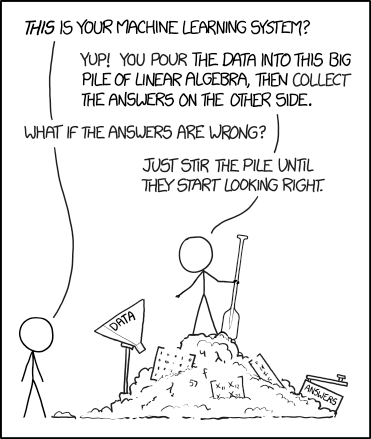
\includegraphics[width=5cm]{img/1838} \pause
			\end{center}
		\end{column}
		\begin{column}{0.5\textwidth}
			Interpretability within Machine Learning is the \textbf{degree} to which we can understand the \textbf{cause} of a decision, and use it to consistently \underline{predict the model's prediction}. \pause \newline \\

			Traditionally, interpretability \& performance is seen as a trade-off.\footnote{sd} \pause \newline \\

			Our work demonstrates a deep intersect between these two \textit{seemingly} orthogonal research foci.
		\end{column}
	\end{columns}
\end{frame}

\section{The Approach}
\begin{frame}{Contrastive Activation Maps}
	HiResCAMs are a \underline{provably faithful} interpretability technique:
	\begin{gather}
		\mathcal{A}^{\text{HiResCAMs}}_{c} = \sum^{F}_{f=1} \frac{\partial \hat{y}_c}{\partial A_f} \odot A_f
	\end{gather} \pause

	Provably faithful because:
	\begin{gather}
		\hat{y}_c = \sum^{D_1, D_2}_{d_1 = 1, d_2 = 1} \mathcal{A}^{\text{HiResCAMs}}_{c, d_1, d_2} + b_c
	\end{gather} \pause
	However, softmax-activated multi-class classification relies on \textbf{inter-class logit differences${}^{!!!}$}, while HiResCAMs re-construct \textit{absolute values}.
\end{frame}

\begin{frame}{Contrastive Activation Maps}
	Therefore, we define \textbf{ContrastiveCAMs}:
	\begin{gather}
			\tilde{\mathcal{\bm{A}}}^{\text{contrastive}}_{(c_t, c_{t'})} := \left\{\tilde{\mathcal{\bm{A}}}_{c_t}^{\text{HiResCAM}} - \tilde{\mathcal{\bm{A}}}_{c_{t'}}^{\text{HiResCAM}}\right\}^{|c|-1}_{c_{t'} \in c \setminus c_t}
	\end{gather}
	This creates a new objective function, equivalent to cross-entropy:\footnote{with subtle changes to the architecture}
	\begin{gather}
		\max_{\theta} \sum^{D_1,D_2}_{d_1,d_2}\tilde{\mathcal{\bm{A}}}_{(c, c'),d_1,d_2}^{\text{contrastive}}\ \forall c' \in \mathbb{Z}_{+}(|c| - 1)
	\end{gather}
	With one key difference: we've preserved spatial information.
\end{frame}

\begin{frame}{The Fault in Our Cross-Entropy}
\end{frame}

\section{Results \& What's Next}
\begin{frame}{Results (so far)}
\end{frame}

\begin{frame}{What's to Come}
	Next, we are going 
\end{frame}

\begin{frame}{Thank you!}
	\begin{center}
		Have an awesome rest of your day!
	\end{center}
	\begin{center}
		\small
		\textbf{Slides:} \url{https://cs.purdue.edu/homes/jsetpal/slides/cont-opt.pdf} \\
		\textbf{Code:} \url{https://dagshub.com/jinensetpal/contrastive-optimization}
	\end{center}
\end{frame}

\end{document}
